% Paper A -- ACIIDS 2027 submission draft (Springer LNCS/LNAI), method paper, version 2.
% All numbers come from results.tex, generated by make_results.py from repository files.
\documentclass[runningheads]{llncs}
\usepackage[T1]{fontenc}
\usepackage{graphicx}
\usepackage{amsmath,amssymb}
\usepackage{booktabs}
\usepackage{xcolor}
\usepackage{algorithm}
\usepackage[noend]{algpseudocode}
\usepackage[hidelinks]{hyperref}
\newif\ifpendshort
% \PENDING{key}: placeholder for a value that does not exist yet (RIS-relevant pilot, NSGA-II).
\newcommand{\PENDING}[1]{\textcolor{red}{\textbf{\ifpendshort P\else[#1]\fi}}}
% AUTO-GENERATED by make_results.py -- do not edit by hand.
% Sources: N=natural-scope leverage diagnostic (validation), G=ME-GA record / pair counts,
% P=production docs, V=v3 scope declaration, S=v3 search declaration, B=benchmark summary (--bench), PENDING=not yet produced.
\providecommand{\PENDING}[1]{\textcolor{red}{\textbf{[#1]}}}
\makeatletter
\newcommand{\res}[1]{\ifcsname res@#1\endcsname\csname res@#1\endcsname\else\PENDING{undefined:#1}\fi}
\expandafter\def\csname res@natApW64\endcsname{0.20}% N
\expandafter\def\csname res@natApH64\endcsname{0.21}% N
\expandafter\def\csname res@natApW128\endcsname{0.42}% N
\expandafter\def\csname res@natApH128\endcsname{0.21}% N
\expandafter\def\csname res@natApW256\endcsname{0.42}% N
\expandafter\def\csname res@natApH256\endcsname{0.45}% N
\expandafter\def\csname res@natFrames64\endcsname{864}% N
\expandafter\def\csname res@natZeroShare64\endcsname{49.1}% N
\expandafter\def\csname res@natZeroBoth64\endcsname{370}% N
\expandafter\def\csname res@natZeroTraj64\endcsname{23}% N
\expandafter\def\csname res@natTraj64\endcsname{54}% N
\expandafter\def\csname res@natOffMinusNoRis64\endcsname{+0.019}% N
\expandafter\def\csname res@natGainAllMean64\endcsname{0.026}% N
\expandafter\def\csname res@natGainAllMedian64\endcsname{0.000}% N
\expandafter\def\csname res@natGainNzMean64\endcsname{0.051}% N
\expandafter\def\csname res@natGainNzMedian64\endcsname{0.015}% N
\expandafter\def\csname res@natGainNzPninety64\endcsname{0.139}% N
\expandafter\def\csname res@natGainNzMax64\endcsname{0.674}% N
\expandafter\def\csname res@natGainGtOne64\endcsname{6.7}% N
\expandafter\def\csname res@natGainGtFive64\endcsname{0.6}% N
\expandafter\def\csname res@natRateOffMean64\endcsname{3.234}% N
\expandafter\def\csname res@natRateNoRisMean64\endcsname{3.215}% N
\expandafter\def\csname res@natRateBestMean64\endcsname{3.260}% N
\expandafter\def\csname res@natRateOnMean64\endcsname{3.181}% N
\expandafter\def\csname res@natRateBestOwnMean64\endcsname{3.253}% N
\expandafter\def\csname res@natIN64\endcsname{$-$6.9}% N
\expandafter\def\csname res@natPrecErr64\endcsname{0}% N
\expandafter\def\csname res@natRisDirBlkLos64\endcsname{$-$55.6}% N
\expandafter\def\csname res@natBoundBlkLos64\endcsname{$-$41.6}% N
\expandafter\def\csname res@natUFBlkLos64\endcsname{340}% N
\expandafter\def\csname res@natRisDirRefLos64\endcsname{$-$55.7}% N
\expandafter\def\csname res@natBoundRefLos64\endcsname{$-$43.2}% N
\expandafter\def\csname res@natUFRefLos64\endcsname{350}% N
\expandafter\def\csname res@natRisDirLosLos64\endcsname{$-$59.2}% N
\expandafter\def\csname res@natBoundLosLos64\endcsname{$-$40.8}% N
\expandafter\def\csname res@natUFLosLos64\endcsname{969}% N
\expandafter\def\csname res@natRisDirBlkRef64\endcsname{+19.6}% N
\expandafter\def\csname res@natBoundBlkRef64\endcsname{$-$41.9}% N
\expandafter\def\csname res@natUFBlkRef64\endcsname{18}% N
\expandafter\def\csname res@natHrNLosLos64\endcsname{136}% N
\expandafter\def\csname res@natHrMedLosLos64\endcsname{0.027}% N
\expandafter\def\csname res@natHrGtLosLos64\endcsname{17}% N
\expandafter\def\csname res@natHrNBlkLos64\endcsname{115}% N
\expandafter\def\csname res@natHrMedBlkLos64\endcsname{0.023}% N
\expandafter\def\csname res@natHrGtBlkLos64\endcsname{24}% N
\expandafter\def\csname res@natZeroMunich64\endcsname{56}% N
\expandafter\def\csname res@natZeroRotterdam64\endcsname{28}% N
\expandafter\def\csname res@natZeroMaastricht64\endcsname{64}% N
\expandafter\def\csname res@natFrames128\endcsname{864}% N
\expandafter\def\csname res@natZeroShare128\endcsname{49.1}% N
\expandafter\def\csname res@natZeroBoth128\endcsname{376}% N
\expandafter\def\csname res@natZeroTraj128\endcsname{23}% N
\expandafter\def\csname res@natTraj128\endcsname{54}% N
\expandafter\def\csname res@natOffMinusNoRis128\endcsname{+0.025}% N
\expandafter\def\csname res@natGainAllMean128\endcsname{0.035}% N
\expandafter\def\csname res@natGainAllMedian128\endcsname{0.000}% N
\expandafter\def\csname res@natGainNzMean128\endcsname{0.069}% N
\expandafter\def\csname res@natGainNzMedian128\endcsname{0.022}% N
\expandafter\def\csname res@natGainNzPninety128\endcsname{0.170}% N
\expandafter\def\csname res@natGainNzMax128\endcsname{0.831}% N
\expandafter\def\csname res@natGainGtOne128\endcsname{10.1}% N
\expandafter\def\csname res@natGainGtFive128\endcsname{1.2}% N
\expandafter\def\csname res@natRateOffMean128\endcsname{3.315}% N
\expandafter\def\csname res@natRateNoRisMean128\endcsname{3.290}% N
\expandafter\def\csname res@natRateBestMean128\endcsname{3.350}% N
\expandafter\def\csname res@natRateOnMean128\endcsname{3.240}% N
\expandafter\def\csname res@natRateBestOwnMean128\endcsname{3.344}% N
\expandafter\def\csname res@natIN128\endcsname{$-$2.6}% N
\expandafter\def\csname res@natPrecErr128\endcsname{0}% N
\expandafter\def\csname res@natRisDirBlkLos128\endcsname{$-$52.8}% N
\expandafter\def\csname res@natBoundBlkLos128\endcsname{$-$36.0}% N
\expandafter\def\csname res@natUFBlkLos128\endcsname{333}% N
\expandafter\def\csname res@natRisDirRefLos128\endcsname{$-$49.6}% N
\expandafter\def\csname res@natBoundRefLos128\endcsname{$-$36.5}% N
\expandafter\def\csname res@natUFRefLos128\endcsname{358}% N
\expandafter\def\csname res@natRisDirLosLos128\endcsname{$-$57.6}% N
\expandafter\def\csname res@natBoundLosLos128\endcsname{$-$34.2}% N
\expandafter\def\csname res@natUFLosLos128\endcsname{972}% N
\expandafter\def\csname res@natRisDirBlkRef128\endcsname{+19.4}% N
\expandafter\def\csname res@natBoundBlkRef128\endcsname{$-$35.2}% N
\expandafter\def\csname res@natUFBlkRef128\endcsname{18}% N
\expandafter\def\csname res@natHrNLosLos128\endcsname{118}% N
\expandafter\def\csname res@natHrMedLosLos128\endcsname{0.050}% N
\expandafter\def\csname res@natHrGtLosLos128\endcsname{33}% N
\expandafter\def\csname res@natHrNBlkLos128\endcsname{104}% N
\expandafter\def\csname res@natHrMedBlkLos128\endcsname{0.029}% N
\expandafter\def\csname res@natHrGtBlkLos128\endcsname{27}% N
\expandafter\def\csname res@natZeroMunich128\endcsname{56}% N
\expandafter\def\csname res@natZeroRotterdam128\endcsname{28}% N
\expandafter\def\csname res@natZeroMaastricht128\endcsname{64}% N
\expandafter\def\csname res@natFrames256\endcsname{864}% N
\expandafter\def\csname res@natZeroShare256\endcsname{49.7}% N
\expandafter\def\csname res@natZeroBoth256\endcsname{381}% N
\expandafter\def\csname res@natZeroTraj256\endcsname{23}% N
\expandafter\def\csname res@natTraj256\endcsname{54}% N
\expandafter\def\csname res@natOffMinusNoRis256\endcsname{+0.043}% N
\expandafter\def\csname res@natGainAllMean256\endcsname{0.060}% N
\expandafter\def\csname res@natGainAllMedian256\endcsname{0.000}% N
\expandafter\def\csname res@natGainNzMean256\endcsname{0.120}% N
\expandafter\def\csname res@natGainNzMedian256\endcsname{0.045}% N
\expandafter\def\csname res@natGainNzPninety256\endcsname{0.292}% N
\expandafter\def\csname res@natGainNzMax256\endcsname{1.488}% N
\expandafter\def\csname res@natGainGtOne256\endcsname{16.3}% N
\expandafter\def\csname res@natGainGtFive256\endcsname{2.8}% N
\expandafter\def\csname res@natRateOffMean256\endcsname{3.242}% N
\expandafter\def\csname res@natRateNoRisMean256\endcsname{3.199}% N
\expandafter\def\csname res@natRateBestMean256\endcsname{3.303}% N
\expandafter\def\csname res@natRateOnMean256\endcsname{3.137}% N
\expandafter\def\csname res@natRateBestOwnMean256\endcsname{3.293}% N
\expandafter\def\csname res@natIN256\endcsname{$-$7.2}% N
\expandafter\def\csname res@natPrecErr256\endcsname{0}% N
\expandafter\def\csname res@natRisDirBlkLos256\endcsname{$-$40.9}% N
\expandafter\def\csname res@natBoundBlkLos256\endcsname{$-$29.4}% N
\expandafter\def\csname res@natUFBlkLos256\endcsname{345}% N
\expandafter\def\csname res@natRisDirRefLos256\endcsname{$-$43.8}% N
\expandafter\def\csname res@natBoundRefLos256\endcsname{$-$29.2}% N
\expandafter\def\csname res@natUFRefLos256\endcsname{346}% N
\expandafter\def\csname res@natRisDirLosLos256\endcsname{$-$56.0}% N
\expandafter\def\csname res@natBoundLosLos256\endcsname{$-$27.6}% N
\expandafter\def\csname res@natUFLosLos256\endcsname{972}% N
\expandafter\def\csname res@natRisDirBlkRef256\endcsname{+19.6}% N
\expandafter\def\csname res@natBoundBlkRef256\endcsname{$-$28.6}% N
\expandafter\def\csname res@natUFBlkRef256\endcsname{18}% N
\expandafter\def\csname res@natHrNLosLos256\endcsname{110}% N
\expandafter\def\csname res@natHrMedLosLos256\endcsname{0.125}% N
\expandafter\def\csname res@natHrGtLosLos256\endcsname{55}% N
\expandafter\def\csname res@natHrNBlkLos256\endcsname{140}% N
\expandafter\def\csname res@natHrMedBlkLos256\endcsname{0.047}% N
\expandafter\def\csname res@natHrGtBlkLos256\endcsname{35}% N
\expandafter\def\csname res@natZeroMunich256\endcsname{56}% N
\expandafter\def\csname res@natZeroRotterdam256\endcsname{28}% N
\expandafter\def\csname res@natZeroMaastricht256\endcsname{65}% N
\expandafter\def\csname res@natFramesTotal\endcsname{2,592}% N
\expandafter\def\csname res@freqGHz\endcsname{5.53}% N
\expandafter\def\csname res@lambdaMm\endcsname{54.2}% N
\expandafter\def\csname res@boundXtenDb\endcsname{11}% N
\expandafter\def\csname res@natDbsrisMedian\endcsname{112}% N
\expandafter\def\csname res@natDbsrisMax\endcsname{150}% N
\expandafter\def\csname res@natDrisUserLo\endcsname{63}% N
\expandafter\def\csname res@natDrisUserHi\endcsname{136}% N
\expandafter\def\csname res@prodTrajPerMap\endcsname{120}% P
\expandafter\def\csname res@prodTraj\endcsname{360}% P
\expandafter\def\csname res@prodFramesPerTraj\endcsname{16}% P
\expandafter\def\csname res@prodFrames\endcsname{5,760}% P
\expandafter\def\csname res@prodArrayFrames\endcsname{17,280}% P
\expandafter\def\csname res@prodValTraj\endcsname{54}% P
\expandafter\def\csname res@siteDminNat\endcsname{20}% P
\expandafter\def\csname res@siteDmaxNat\endcsname{150}% P
\expandafter\def\csname res@negSlotProb\endcsname{0.15}% P
\expandafter\def\csname res@rtSamples\endcsname{10,000}% P
\expandafter\def\csname res@rtDepth\endcsname{2}% P
\expandafter\def\csname res@openGapPct\endcsname{4.7}% P
\expandafter\def\csname res@megaPop\endcsname{100}% G
\expandafter\def\csname res@megaIter\endcsname{100}% G
\expandafter\def\csname res@megaDecisions\endcsname{24}% G
\expandafter\def\csname res@megaSensItems\endcsname{9}% G
\expandafter\def\csname res@nPairsSixtyFour\endcsname{2,016}% G
\expandafter\def\csname res@nPairsOneTwentyEight\endcsname{8,128}% G
\expandafter\def\csname res@nPairsTwoFiftySix\endcsname{32,640}% G
\expandafter\def\csname res@megaWoodM\endcsname{24}% G
\expandafter\def\csname res@megaWoodMin\endcsname{12}% G
\expandafter\def\csname res@nsgaPop\endcsname{20}% G
\expandafter\def\csname res@nsgaPc\endcsname{0.9}% G
\expandafter\def\csname res@nsgaGridP\endcsname{20/50/100}% G
\expandafter\def\csname res@nsgaGridPc\endcsname{0.7/0.9}% G
\expandafter\def\csname res@nsgaGridN\endcsname{6}% G
\expandafter\def\csname res@vMap\endcsname{Rotterdam}% V
\expandafter\def\csname res@vTraj\endcsname{120}% V
\expandafter\def\csname res@vFrames\endcsname{16}% V
\expandafter\def\csname res@vTrainTraj\endcsname{84}% V
\expandafter\def\csname res@vValTraj\endcsname{18}% V
\expandafter\def\csname res@vTestTraj\endcsname{18}% V
\expandafter\def\csname res@vDmin\endcsname{5}% V
\expandafter\def\csname res@vDmax\endcsname{20}% V
\expandafter\def\csname res@vDOneMin\endcsname{7.8}% V
\expandafter\def\csname res@vDOneMed\endcsname{13.7}% V
\expandafter\def\csname res@vDOneMax\endcsname{18.7}% V
\expandafter\def\csname res@vSites\endcsname{4}% V
\expandafter\def\csname res@vDTwoLo\endcsname{26.7}% V
\expandafter\def\csname res@vDTwoMed\endcsname{32.3}% V
\expandafter\def\csname res@vDTwoHi\endcsname{36.4}% V
\expandafter\def\csname res@vRadius\endcsname{40}% V
\expandafter\def\csname res@vAngle\endcsname{80}% V
\expandafter\def\csname res@vServedUF\endcsname{4,800}% V
\expandafter\def\csname res@vSamples\endcsname{10^{6}}% V
\expandafter\def\csname res@vPathCap\endcsname{2\times10^{6}}% V
\expandafter\def\csname res@vDepth\endcsname{2}% V
\expandafter\def\csname res@vUnitsOk\endcsname{357}% V
\expandafter\def\csname res@vUnits\endcsname{360}% V
\expandafter\def\csname res@vIncluded\endcsname{119}% V
\expandafter\def\csname res@vGainMed64\endcsname{0.302}% V
\expandafter\def\csname res@vGainMed128\endcsname{0.418}% V
\expandafter\def\csname res@vGainMed256\endcsname{0.782}% V
\expandafter\def\csname res@vGainMean64\endcsname{0.450}% V
\expandafter\def\csname res@vGainPninety64\endcsname{1.089}% V
\expandafter\def\csname res@vGainMean128\endcsname{0.534}% V
\expandafter\def\csname res@vGainPninety128\endcsname{1.379}% V
\expandafter\def\csname res@vGainMean256\endcsname{1.097}% V
\expandafter\def\csname res@vGainPninety256\endcsname{2.760}% V
\expandafter\def\csname res@vPathless\endcsname{0.0}% V
\expandafter\def\csname res@vSeeds\endcsname{10}% S
\expandafter\def\csname res@vBoot\endcsname{10,000}% S
\expandafter\def\csname res@vFamily\endcsname{five}% S
\expandafter\def\csname res@vMaxMiss\endcsname{0.5}% S
\expandafter\def\csname res@vRateGreedyFive64\endcsname{\PENDING{vRateGreedyFive64}}% PENDING
\expandafter\def\csname res@vRateGreedyTen64\endcsname{\PENDING{vRateGreedyTen64}}% PENDING
\expandafter\def\csname res@vRateGreedyFifty64\endcsname{\PENDING{vRateGreedyFifty64}}% PENDING
\expandafter\def\csname res@vRateGreedyHundred64\endcsname{\PENDING{vRateGreedyHundred64}}% PENDING
\expandafter\def\csname res@vLatGreedy64\endcsname{\PENDING{vLatGreedy64}}% PENDING
\expandafter\def\csname res@vLatPGreedy64\endcsname{\PENDING{vLatPGreedy64}}% PENDING
\expandafter\def\csname res@vEvalsGreedy64\endcsname{\PENDING{vEvalsGreedy64}}% PENDING
\expandafter\def\csname res@vMissGreedy64\endcsname{\PENDING{vMissGreedy64}}% PENDING
\expandafter\def\csname res@vRatePairFive64\endcsname{\PENDING{vRatePairFive64}}% PENDING
\expandafter\def\csname res@vRatePairTen64\endcsname{\PENDING{vRatePairTen64}}% PENDING
\expandafter\def\csname res@vRatePairFifty64\endcsname{\PENDING{vRatePairFifty64}}% PENDING
\expandafter\def\csname res@vRatePairHundred64\endcsname{\PENDING{vRatePairHundred64}}% PENDING
\expandafter\def\csname res@vLatPair64\endcsname{\PENDING{vLatPair64}}% PENDING
\expandafter\def\csname res@vLatPPair64\endcsname{\PENDING{vLatPPair64}}% PENDING
\expandafter\def\csname res@vEvalsPair64\endcsname{\PENDING{vEvalsPair64}}% PENDING
\expandafter\def\csname res@vMissPair64\endcsname{\PENDING{vMissPair64}}% PENDING
\expandafter\def\csname res@vRateBthreeFive64\endcsname{\PENDING{vRateBthreeFive64}}% PENDING
\expandafter\def\csname res@vRateBthreeTen64\endcsname{\PENDING{vRateBthreeTen64}}% PENDING
\expandafter\def\csname res@vRateBthreeFifty64\endcsname{\PENDING{vRateBthreeFifty64}}% PENDING
\expandafter\def\csname res@vRateBthreeHundred64\endcsname{\PENDING{vRateBthreeHundred64}}% PENDING
\expandafter\def\csname res@vLatBthree64\endcsname{\PENDING{vLatBthree64}}% PENDING
\expandafter\def\csname res@vLatPBthree64\endcsname{\PENDING{vLatPBthree64}}% PENDING
\expandafter\def\csname res@vEvalsBthree64\endcsname{\PENDING{vEvalsBthree64}}% PENDING
\expandafter\def\csname res@vMissBthree64\endcsname{\PENDING{vMissBthree64}}% PENDING
\expandafter\def\csname res@vRateBfiveFive64\endcsname{\PENDING{vRateBfiveFive64}}% PENDING
\expandafter\def\csname res@vRateBfiveTen64\endcsname{\PENDING{vRateBfiveTen64}}% PENDING
\expandafter\def\csname res@vRateBfiveFifty64\endcsname{\PENDING{vRateBfiveFifty64}}% PENDING
\expandafter\def\csname res@vRateBfiveHundred64\endcsname{\PENDING{vRateBfiveHundred64}}% PENDING
\expandafter\def\csname res@vLatBfive64\endcsname{\PENDING{vLatBfive64}}% PENDING
\expandafter\def\csname res@vLatPBfive64\endcsname{\PENDING{vLatPBfive64}}% PENDING
\expandafter\def\csname res@vEvalsBfive64\endcsname{\PENDING{vEvalsBfive64}}% PENDING
\expandafter\def\csname res@vMissBfive64\endcsname{\PENDING{vMissBfive64}}% PENDING
\expandafter\def\csname res@vRateBtsFive64\endcsname{\PENDING{vRateBtsFive64}}% PENDING
\expandafter\def\csname res@vRateBtsTen64\endcsname{\PENDING{vRateBtsTen64}}% PENDING
\expandafter\def\csname res@vRateBtsFifty64\endcsname{\PENDING{vRateBtsFifty64}}% PENDING
\expandafter\def\csname res@vRateBtsHundred64\endcsname{\PENDING{vRateBtsHundred64}}% PENDING
\expandafter\def\csname res@vLatBts64\endcsname{\PENDING{vLatBts64}}% PENDING
\expandafter\def\csname res@vLatPBts64\endcsname{\PENDING{vLatPBts64}}% PENDING
\expandafter\def\csname res@vEvalsBts64\endcsname{\PENDING{vEvalsBts64}}% PENDING
\expandafter\def\csname res@vMissBts64\endcsname{\PENDING{vMissBts64}}% PENDING
\expandafter\def\csname res@vRateMegaFive64\endcsname{\PENDING{vRateMegaFive64}}% PENDING
\expandafter\def\csname res@vRateMegaTen64\endcsname{\PENDING{vRateMegaTen64}}% PENDING
\expandafter\def\csname res@vRateMegaFifty64\endcsname{\PENDING{vRateMegaFifty64}}% PENDING
\expandafter\def\csname res@vRateMegaHundred64\endcsname{\PENDING{vRateMegaHundred64}}% PENDING
\expandafter\def\csname res@vLatMega64\endcsname{\PENDING{vLatMega64}}% PENDING
\expandafter\def\csname res@vLatPMega64\endcsname{\PENDING{vLatPMega64}}% PENDING
\expandafter\def\csname res@vEvalsMega64\endcsname{\PENDING{vEvalsMega64}}% PENDING
\expandafter\def\csname res@vMissMega64\endcsname{\PENDING{vMissMega64}}% PENDING
\expandafter\def\csname res@vRateNsgaFive64\endcsname{\PENDING{vRateNsgaFive64}}% PENDING
\expandafter\def\csname res@vRateNsgaTen64\endcsname{\PENDING{vRateNsgaTen64}}% PENDING
\expandafter\def\csname res@vRateNsgaFifty64\endcsname{\PENDING{vRateNsgaFifty64}}% PENDING
\expandafter\def\csname res@vRateNsgaHundred64\endcsname{\PENDING{vRateNsgaHundred64}}% PENDING
\expandafter\def\csname res@vLatNsga64\endcsname{\PENDING{vLatNsga64}}% PENDING
\expandafter\def\csname res@vLatPNsga64\endcsname{\PENDING{vLatPNsga64}}% PENDING
\expandafter\def\csname res@vEvalsNsga64\endcsname{\PENDING{vEvalsNsga64}}% PENDING
\expandafter\def\csname res@vMissNsga64\endcsname{\PENDING{vMissNsga64}}% PENDING
\expandafter\def\csname res@vHOne64\endcsname{\PENDING{vHOne64}}% PENDING
\expandafter\def\csname res@vHOneVerdict64\endcsname{\PENDING{vHOneVerdict64}}% PENDING
\expandafter\def\csname res@vHTwo64\endcsname{\PENDING{vHTwo64}}% PENDING
\expandafter\def\csname res@vHTwoVerdict64\endcsname{\PENDING{vHTwoVerdict64}}% PENDING
\expandafter\def\csname res@vHFive64\endcsname{\PENDING{vHFive64}}% PENDING
\expandafter\def\csname res@vHFiveVerdict64\endcsname{\PENDING{vHFiveVerdict64}}% PENDING
\expandafter\def\csname res@vRateGreedyFive128\endcsname{\PENDING{vRateGreedyFive128}}% PENDING
\expandafter\def\csname res@vRateGreedyTen128\endcsname{\PENDING{vRateGreedyTen128}}% PENDING
\expandafter\def\csname res@vRateGreedyFifty128\endcsname{\PENDING{vRateGreedyFifty128}}% PENDING
\expandafter\def\csname res@vRateGreedyHundred128\endcsname{\PENDING{vRateGreedyHundred128}}% PENDING
\expandafter\def\csname res@vLatGreedy128\endcsname{\PENDING{vLatGreedy128}}% PENDING
\expandafter\def\csname res@vLatPGreedy128\endcsname{\PENDING{vLatPGreedy128}}% PENDING
\expandafter\def\csname res@vEvalsGreedy128\endcsname{\PENDING{vEvalsGreedy128}}% PENDING
\expandafter\def\csname res@vMissGreedy128\endcsname{\PENDING{vMissGreedy128}}% PENDING
\expandafter\def\csname res@vRatePairFive128\endcsname{\PENDING{vRatePairFive128}}% PENDING
\expandafter\def\csname res@vRatePairTen128\endcsname{\PENDING{vRatePairTen128}}% PENDING
\expandafter\def\csname res@vRatePairFifty128\endcsname{\PENDING{vRatePairFifty128}}% PENDING
\expandafter\def\csname res@vRatePairHundred128\endcsname{\PENDING{vRatePairHundred128}}% PENDING
\expandafter\def\csname res@vLatPair128\endcsname{\PENDING{vLatPair128}}% PENDING
\expandafter\def\csname res@vLatPPair128\endcsname{\PENDING{vLatPPair128}}% PENDING
\expandafter\def\csname res@vEvalsPair128\endcsname{\PENDING{vEvalsPair128}}% PENDING
\expandafter\def\csname res@vMissPair128\endcsname{\PENDING{vMissPair128}}% PENDING
\expandafter\def\csname res@vRateBthreeFive128\endcsname{\PENDING{vRateBthreeFive128}}% PENDING
\expandafter\def\csname res@vRateBthreeTen128\endcsname{\PENDING{vRateBthreeTen128}}% PENDING
\expandafter\def\csname res@vRateBthreeFifty128\endcsname{\PENDING{vRateBthreeFifty128}}% PENDING
\expandafter\def\csname res@vRateBthreeHundred128\endcsname{\PENDING{vRateBthreeHundred128}}% PENDING
\expandafter\def\csname res@vLatBthree128\endcsname{\PENDING{vLatBthree128}}% PENDING
\expandafter\def\csname res@vLatPBthree128\endcsname{\PENDING{vLatPBthree128}}% PENDING
\expandafter\def\csname res@vEvalsBthree128\endcsname{\PENDING{vEvalsBthree128}}% PENDING
\expandafter\def\csname res@vMissBthree128\endcsname{\PENDING{vMissBthree128}}% PENDING
\expandafter\def\csname res@vRateBfiveFive128\endcsname{\PENDING{vRateBfiveFive128}}% PENDING
\expandafter\def\csname res@vRateBfiveTen128\endcsname{\PENDING{vRateBfiveTen128}}% PENDING
\expandafter\def\csname res@vRateBfiveFifty128\endcsname{\PENDING{vRateBfiveFifty128}}% PENDING
\expandafter\def\csname res@vRateBfiveHundred128\endcsname{\PENDING{vRateBfiveHundred128}}% PENDING
\expandafter\def\csname res@vLatBfive128\endcsname{\PENDING{vLatBfive128}}% PENDING
\expandafter\def\csname res@vLatPBfive128\endcsname{\PENDING{vLatPBfive128}}% PENDING
\expandafter\def\csname res@vEvalsBfive128\endcsname{\PENDING{vEvalsBfive128}}% PENDING
\expandafter\def\csname res@vMissBfive128\endcsname{\PENDING{vMissBfive128}}% PENDING
\expandafter\def\csname res@vRateBtsFive128\endcsname{\PENDING{vRateBtsFive128}}% PENDING
\expandafter\def\csname res@vRateBtsTen128\endcsname{\PENDING{vRateBtsTen128}}% PENDING
\expandafter\def\csname res@vRateBtsFifty128\endcsname{\PENDING{vRateBtsFifty128}}% PENDING
\expandafter\def\csname res@vRateBtsHundred128\endcsname{\PENDING{vRateBtsHundred128}}% PENDING
\expandafter\def\csname res@vLatBts128\endcsname{\PENDING{vLatBts128}}% PENDING
\expandafter\def\csname res@vLatPBts128\endcsname{\PENDING{vLatPBts128}}% PENDING
\expandafter\def\csname res@vEvalsBts128\endcsname{\PENDING{vEvalsBts128}}% PENDING
\expandafter\def\csname res@vMissBts128\endcsname{\PENDING{vMissBts128}}% PENDING
\expandafter\def\csname res@vRateMegaFive128\endcsname{\PENDING{vRateMegaFive128}}% PENDING
\expandafter\def\csname res@vRateMegaTen128\endcsname{\PENDING{vRateMegaTen128}}% PENDING
\expandafter\def\csname res@vRateMegaFifty128\endcsname{\PENDING{vRateMegaFifty128}}% PENDING
\expandafter\def\csname res@vRateMegaHundred128\endcsname{\PENDING{vRateMegaHundred128}}% PENDING
\expandafter\def\csname res@vLatMega128\endcsname{\PENDING{vLatMega128}}% PENDING
\expandafter\def\csname res@vLatPMega128\endcsname{\PENDING{vLatPMega128}}% PENDING
\expandafter\def\csname res@vEvalsMega128\endcsname{\PENDING{vEvalsMega128}}% PENDING
\expandafter\def\csname res@vMissMega128\endcsname{\PENDING{vMissMega128}}% PENDING
\expandafter\def\csname res@vRateNsgaFive128\endcsname{\PENDING{vRateNsgaFive128}}% PENDING
\expandafter\def\csname res@vRateNsgaTen128\endcsname{\PENDING{vRateNsgaTen128}}% PENDING
\expandafter\def\csname res@vRateNsgaFifty128\endcsname{\PENDING{vRateNsgaFifty128}}% PENDING
\expandafter\def\csname res@vRateNsgaHundred128\endcsname{\PENDING{vRateNsgaHundred128}}% PENDING
\expandafter\def\csname res@vLatNsga128\endcsname{\PENDING{vLatNsga128}}% PENDING
\expandafter\def\csname res@vLatPNsga128\endcsname{\PENDING{vLatPNsga128}}% PENDING
\expandafter\def\csname res@vEvalsNsga128\endcsname{\PENDING{vEvalsNsga128}}% PENDING
\expandafter\def\csname res@vMissNsga128\endcsname{\PENDING{vMissNsga128}}% PENDING
\expandafter\def\csname res@vHOne128\endcsname{\PENDING{vHOne128}}% PENDING
\expandafter\def\csname res@vHOneVerdict128\endcsname{\PENDING{vHOneVerdict128}}% PENDING
\expandafter\def\csname res@vHTwo128\endcsname{\PENDING{vHTwo128}}% PENDING
\expandafter\def\csname res@vHTwoVerdict128\endcsname{\PENDING{vHTwoVerdict128}}% PENDING
\expandafter\def\csname res@vHFive128\endcsname{\PENDING{vHFive128}}% PENDING
\expandafter\def\csname res@vHFiveVerdict128\endcsname{\PENDING{vHFiveVerdict128}}% PENDING
\expandafter\def\csname res@vRateGreedyFive256\endcsname{\PENDING{vRateGreedyFive256}}% PENDING
\expandafter\def\csname res@vRateGreedyTen256\endcsname{\PENDING{vRateGreedyTen256}}% PENDING
\expandafter\def\csname res@vRateGreedyFifty256\endcsname{\PENDING{vRateGreedyFifty256}}% PENDING
\expandafter\def\csname res@vRateGreedyHundred256\endcsname{\PENDING{vRateGreedyHundred256}}% PENDING
\expandafter\def\csname res@vLatGreedy256\endcsname{\PENDING{vLatGreedy256}}% PENDING
\expandafter\def\csname res@vLatPGreedy256\endcsname{\PENDING{vLatPGreedy256}}% PENDING
\expandafter\def\csname res@vEvalsGreedy256\endcsname{\PENDING{vEvalsGreedy256}}% PENDING
\expandafter\def\csname res@vMissGreedy256\endcsname{\PENDING{vMissGreedy256}}% PENDING
\expandafter\def\csname res@vRatePairFive256\endcsname{\PENDING{vRatePairFive256}}% PENDING
\expandafter\def\csname res@vRatePairTen256\endcsname{\PENDING{vRatePairTen256}}% PENDING
\expandafter\def\csname res@vRatePairFifty256\endcsname{\PENDING{vRatePairFifty256}}% PENDING
\expandafter\def\csname res@vRatePairHundred256\endcsname{\PENDING{vRatePairHundred256}}% PENDING
\expandafter\def\csname res@vLatPair256\endcsname{\PENDING{vLatPair256}}% PENDING
\expandafter\def\csname res@vLatPPair256\endcsname{\PENDING{vLatPPair256}}% PENDING
\expandafter\def\csname res@vEvalsPair256\endcsname{\PENDING{vEvalsPair256}}% PENDING
\expandafter\def\csname res@vMissPair256\endcsname{\PENDING{vMissPair256}}% PENDING
\expandafter\def\csname res@vRateBthreeFive256\endcsname{\PENDING{vRateBthreeFive256}}% PENDING
\expandafter\def\csname res@vRateBthreeTen256\endcsname{\PENDING{vRateBthreeTen256}}% PENDING
\expandafter\def\csname res@vRateBthreeFifty256\endcsname{\PENDING{vRateBthreeFifty256}}% PENDING
\expandafter\def\csname res@vRateBthreeHundred256\endcsname{\PENDING{vRateBthreeHundred256}}% PENDING
\expandafter\def\csname res@vLatBthree256\endcsname{\PENDING{vLatBthree256}}% PENDING
\expandafter\def\csname res@vLatPBthree256\endcsname{\PENDING{vLatPBthree256}}% PENDING
\expandafter\def\csname res@vEvalsBthree256\endcsname{\PENDING{vEvalsBthree256}}% PENDING
\expandafter\def\csname res@vMissBthree256\endcsname{\PENDING{vMissBthree256}}% PENDING
\expandafter\def\csname res@vRateBfiveFive256\endcsname{\PENDING{vRateBfiveFive256}}% PENDING
\expandafter\def\csname res@vRateBfiveTen256\endcsname{\PENDING{vRateBfiveTen256}}% PENDING
\expandafter\def\csname res@vRateBfiveFifty256\endcsname{\PENDING{vRateBfiveFifty256}}% PENDING
\expandafter\def\csname res@vRateBfiveHundred256\endcsname{\PENDING{vRateBfiveHundred256}}% PENDING
\expandafter\def\csname res@vLatBfive256\endcsname{\PENDING{vLatBfive256}}% PENDING
\expandafter\def\csname res@vLatPBfive256\endcsname{\PENDING{vLatPBfive256}}% PENDING
\expandafter\def\csname res@vEvalsBfive256\endcsname{\PENDING{vEvalsBfive256}}% PENDING
\expandafter\def\csname res@vMissBfive256\endcsname{\PENDING{vMissBfive256}}% PENDING
\expandafter\def\csname res@vRateBtsFive256\endcsname{\PENDING{vRateBtsFive256}}% PENDING
\expandafter\def\csname res@vRateBtsTen256\endcsname{\PENDING{vRateBtsTen256}}% PENDING
\expandafter\def\csname res@vRateBtsFifty256\endcsname{\PENDING{vRateBtsFifty256}}% PENDING
\expandafter\def\csname res@vRateBtsHundred256\endcsname{\PENDING{vRateBtsHundred256}}% PENDING
\expandafter\def\csname res@vLatBts256\endcsname{\PENDING{vLatBts256}}% PENDING
\expandafter\def\csname res@vLatPBts256\endcsname{\PENDING{vLatPBts256}}% PENDING
\expandafter\def\csname res@vEvalsBts256\endcsname{\PENDING{vEvalsBts256}}% PENDING
\expandafter\def\csname res@vMissBts256\endcsname{\PENDING{vMissBts256}}% PENDING
\expandafter\def\csname res@vRateMegaFive256\endcsname{\PENDING{vRateMegaFive256}}% PENDING
\expandafter\def\csname res@vRateMegaTen256\endcsname{\PENDING{vRateMegaTen256}}% PENDING
\expandafter\def\csname res@vRateMegaFifty256\endcsname{\PENDING{vRateMegaFifty256}}% PENDING
\expandafter\def\csname res@vRateMegaHundred256\endcsname{\PENDING{vRateMegaHundred256}}% PENDING
\expandafter\def\csname res@vLatMega256\endcsname{\PENDING{vLatMega256}}% PENDING
\expandafter\def\csname res@vLatPMega256\endcsname{\PENDING{vLatPMega256}}% PENDING
\expandafter\def\csname res@vEvalsMega256\endcsname{\PENDING{vEvalsMega256}}% PENDING
\expandafter\def\csname res@vMissMega256\endcsname{\PENDING{vMissMega256}}% PENDING
\expandafter\def\csname res@vRateNsgaFive256\endcsname{\PENDING{vRateNsgaFive256}}% PENDING
\expandafter\def\csname res@vRateNsgaTen256\endcsname{\PENDING{vRateNsgaTen256}}% PENDING
\expandafter\def\csname res@vRateNsgaFifty256\endcsname{\PENDING{vRateNsgaFifty256}}% PENDING
\expandafter\def\csname res@vRateNsgaHundred256\endcsname{\PENDING{vRateNsgaHundred256}}% PENDING
\expandafter\def\csname res@vLatNsga256\endcsname{\PENDING{vLatNsga256}}% PENDING
\expandafter\def\csname res@vLatPNsga256\endcsname{\PENDING{vLatPNsga256}}% PENDING
\expandafter\def\csname res@vEvalsNsga256\endcsname{\PENDING{vEvalsNsga256}}% PENDING
\expandafter\def\csname res@vMissNsga256\endcsname{\PENDING{vMissNsga256}}% PENDING
\expandafter\def\csname res@vHOne256\endcsname{\PENDING{vHOne256}}% PENDING
\expandafter\def\csname res@vHOneVerdict256\endcsname{\PENDING{vHOneVerdict256}}% PENDING
\expandafter\def\csname res@vHTwo256\endcsname{\PENDING{vHTwo256}}% PENDING
\expandafter\def\csname res@vHTwoVerdict256\endcsname{\PENDING{vHTwoVerdict256}}% PENDING
\expandafter\def\csname res@vHFive256\endcsname{\PENDING{vHFive256}}% PENDING
\expandafter\def\csname res@vHFiveVerdict256\endcsname{\PENDING{vHFiveVerdict256}}% PENDING
\expandafter\def\csname res@vBenchLoaded\endcsname{no}% B
\makeatother

\newcommand{\bts}{\textsc{b35}}
\newcommand{\Hd}{H_{\mathrm{d}}}
\renewcommand{\algorithmiccomment}[1]{\hfill{\footnotesize$\triangleright$ #1}}

\begin{document}
\title{Title TBD}
\titlerunning{Title TBD}
\author{Author One\inst{1}\orcidID{0000-0000-0000-0000} \and
Author Two\inst{1} \and
Author Three\inst{2}}
\authorrunning{A. One et al.}
\institute{Department, University, City, Country\\
\email{\{author.one,author.two\}@example.edu} \and
Department, Institute, City, Country\\
\email{author.three@example.org}}
\maketitle

\begin{abstract}
Configuring a 1-bit reconfigurable intelligent surface (RIS) to maximise the worst user's rate is a binary max--min problem that must be solved again whenever users move, often within tens of milliseconds. Evolutionary controllers are the usual answer, but each candidate costs a full channel evaluation, and on a mutually coupled surface that evaluation is a matrix inverse. We propose \bts{}, an anytime local search that (i) scores every single and every pair flip exactly through rank-one and rank-two Woodbury updates of the coupled multiport network, (ii) restarts from states drawn at two predeclared ON densities, and (iii) every third restart recombines two cached local optima. All set-up, scans and the final rescore run inside a hard CPU deadline. On a frozen held-out test with a full thin-wire method-of-moments surface model, \bts{} beats exact pair search by \res{fsDBtsPairFifty}\,bit/s/Hz under a 50\,ms deadline (Bonferroni interval [\res{fsLoBtsPairFifty}, \res{fsHiBtsPairFifty}], \res{fsWinsBtsPairFifty} of \res{fsN} trajectories), beats both of its components, and outperforms a reimplementation of the memory-enhanced genetic algorithm ME-GA by \res{fsDBtsMegaFifty}\,bit/s/Hz. The main evaluation is a pre-registered RIS-relevant scope of the GeoRIS-Bench city benchmark, built from LoD2 building models and ray tracing, where \bts{} is compared with exact pair search, ME-GA and NSGA-II at 64, 128 and 256 elements on solution quality, latency and budget.
\keywords{Reconfigurable intelligent surface \and Combinatorial optimisation \and Anytime search \and Local search \and Evolutionary algorithms \and Mutual coupling.}
\end{abstract}

%======================================================================
\section{Introduction}
%======================================================================
A reconfigurable intelligent surface is a passive array whose elements switch between a few load states, so that the field it re-radiates can be shaped without active transmit chains~\cite{li2026tutorial}. With 1-bit elements, configuring an $N$-element surface means choosing one of $2^N$ binary states. When the surface serves several users from a multi-antenna base station (BS), a natural objective is the rate of the worst served user. This objective is non-smooth, and once mutual coupling between elements is modelled~\cite{qian2020mutual,zheng2024mutual,nerini2024universal,nerini2026global}, it is also non-separable: the effect of one element depends on the state of all others. Users move, so the problem must be re-solved every few tens of milliseconds, on the hardware that controls the surface~\cite{urbinati2026ondevice}. The practical question is therefore not which method finds the global optimum, but which method returns the best state \emph{by a fixed deadline}.

Population-based evolutionary algorithms are a common choice for this setting. Zardi, Oliveri and Massa~\cite{zardi2024memory} proposed ME-GA, a genetic algorithm whose memory of earlier good individuals lets it track a changing channel, and multi-objective evolutionary algorithms such as NSGA-II~\cite{deb2002fast} are standard black-box baselines. Their weakness under a deadline is cost: every individual needs a full channel evaluation, which on a coupled surface means inverting an $N\times N$ impedance matrix. Single-flip local search is cheaper, because a flip changes one diagonal load and can be scored by a rank-one update, but it stalls: a state can be optimal with respect to every single flip and still be improved by flipping two coupled elements together. In a free-space coupled reference, \res{vOnePairOpt} of \res{vOneParents} single-flip local optima (\res{vOnePairOptPct}\%) admitted an improving pair.

This paper builds a deadline-bounded search on top of exact pair moves. Its contributions are:
\begin{enumerate}
\item \textbf{\bts{}}, an anytime local search for coupled 1-bit RIS control. It scores all $N$ single flips and all $N(N-1)/2$ pair flips exactly with rank-one and rank-two updates of the coupled network, and diversifies through two predeclared restart densities and elite recombination of cached local optima (Sect.~\ref{sec:method}).
\item \textbf{A deadline-fair evaluation protocol}, in which the clock covers evaluator set-up and every scan, the decision rules are frozen before a single held-out run, and every method faces the same evaluator and deadline (Sect.~\ref{sec:protocol}).
\item \textbf{A city-scale evaluation} on a RIS-relevant scope of GeoRIS-Bench, built from LoD2 building models and ray tracing, against exact pair search, ME-GA and NSGA-II, reported on three metrics shared across methods: worst-user rate, latency and budget (Sect.~\ref{sec:results}); and a frozen held-out controlled check on a free-space surface modelled with the full thin-wire method of moments.
\end{enumerate}

%======================================================================
\section{Related Work}\label{sec:related}
%======================================================================
\textbf{Learning-based configuration.} Deep networks that map channel observations to RIS states have been implemented on FPGAs~\cite{martin2024hardware,padial2026accelerating} and on embedded devices, where the latency--rate trade-off is explicit~\cite{urbinati2026ondevice}. Other works add robustness to practical constraints~\cite{xu2022robust}, account for coupling and partial channel knowledge~\cite{peng2025risnet}, or train generative surrogates on full-wave data~\cite{liu2026physics}. These methods amortise optimisation into training; the present work instead studies search at decision time.

\textbf{Evolutionary and discrete search.} ME-GA~\cite{zardi2024memory} adapts its mutation and crossover rates to population diversity and uses a memory of past best individuals to react to channel changes. NSGA-II~\cite{deb2002fast} is the reference elitist evolutionary algorithm, and learned genetic operators have been obtained by meta-black-box optimisation~\cite{lange2023discovering}. For discrete RIS configuration, Zhang et al.~\cite{zhang2022configuring} gave an algorithm with performance guarantees, and Hammami et al.~\cite{hammami2026statistical} found simple coordinate methods hard to beat on statistical multiport models.

\textbf{Coupled models and efficient updates.} Mutual impedance models~\cite{qian2020mutual}, multiport network frameworks~\cite{nerini2024universal,nossek2024physically}, S-parameter designs with full-wave validation~\cite{abrardo2024design} and closed-form optima under coupling~\cite{nerini2026global} establish the impedance-domain channel used here. PhysFad~\cite{faqiri2023physfad} and Prod'homme and del Hougne~\cite{prodhomme2023efficient} model RIS-parametrised environments with coupled dipoles, and the latter use low-rank updates to compute channel realisations efficiently. We use the same algebra inside a deadline-bounded search, and scan the complete pair neighbourhood at each step. Measured datasets~\cite{tewes2023comprehensive,rossanese2024open,piana2026brisc} and simulators~\cite{burtakov2023qris} supply channels but do not fix a deadline-bounded protocol for comparing configuration methods.

%======================================================================
\section{Problem and Coupled Evaluator}\label{sec:problem}
%======================================================================
\textbf{Channel.} The surface has $N$ thin-wire elements; each is terminated by one of two passive loads $z_0,z_1$ (1\,$\Omega$ resistance, reactances $\pm70\,\Omega$ around the isolated-wire resonance). Let $Z_{\mathrm{RIS}}$ be the full $N\times N$ impedance matrix from NEC-2~\cite{burke1981nec,pynec}, after a Schur-complement reduction over the 50\,$\Omega$-terminated BS and user ports. With $Z_L(\mathbf b)=\mathrm{diag}(z_{b_1},\dots,z_{b_N})$ and $T(\mathbf b)=(Z_{\mathrm{RIS}}+Z_L(\mathbf b))^{-1}$, the channel from the four BS ports to the $K$ users is
\begin{equation}
H(\mathbf b)=\Hd + C_{\mathrm{out}}\,T(\mathbf b)\,C_{\mathrm{in}},
\label{eq:operator}
\end{equation}
where $\Hd$ is the direct channel and $C_{\mathrm{in}}$, $C_{\mathrm{out}}$ couple the elements to the BS and the users. The off-diagonal entries of $Z_{\mathrm{RIS}}$ are the mutual coupling; ignoring them changed predicted rates by \res{fsCoupMae}\,bit/s/Hz in mean absolute terms over \res{fsCoupPatterns} random states of one free-space frame.

\textbf{Objective.} A regularised zero-forcing precoder $W$ is computed once from the all-OFF channel and kept fixed. With effective field $U(\mathbf b)=H(\mathbf b)W$ and noise power $\sigma^2$,
\begin{equation}
\max_{\mathbf b\in\{0,1\}^N} f(\mathbf b),\qquad f(\mathbf b)=\min_{k}\log_2\Bigl(1+\frac{|U_{kk}|^2}{\sum_{j\ne k}|U_{kj}|^2+\sigma^2}\Bigr).
\label{eq:objective}
\end{equation}

\textbf{Exact single and pair moves.} Flipping element $i$ changes one diagonal load by $\delta_i=z_{1-b_i}-z_{b_i}$. Given $T$, precompute $L=C_{\mathrm{out}}T\in\mathbb C^{K\times N}$, $R=TC_{\mathrm{in}}W\in\mathbb C^{N\times S}$ and $d_i=1/\delta_i+T_{ii}$. By Sherman--Morrison, the field after flipping $i$ is
\begin{equation}
U^{(i)}=U-\frac{\ell_i\,r_i^{\top}}{d_i},
\end{equation}
with $\ell_i$ the $i$-th column of $L$ and $r_i^\top$ the $i$-th row of $R$. For a pair $(i,j)$, the $2\times2$ Woodbury identity gives, with $\Delta_{ij}=d_id_j-T_{ij}T_{ji}$,
\begin{equation}
U^{(ij)}=U-\ell_i u_i^{\top}-\ell_j u_j^{\top},\quad u_i=\frac{d_jr_i-T_{ij}r_j}{\Delta_{ij}},\quad u_j=\frac{d_ir_j-T_{ji}r_i}{\Delta_{ij}}.
\label{eq:pair}
\end{equation}
\textbf{Cost.} Forming $L$ and $R$ costs $O(N^2(K+S))$ once per state. Each single move then costs $O(KS)$ and each pair move $O(KS)$ plus a $2\times2$ determinant, so a full scan of all $N(N-1)/2$ pairs costs $O(N^2KS)$. Scoring each pair by a fresh inverse would cost $O(N^3)$ per candidate, i.e.\ $O(N^5)$ per scan. Committing an accepted move updates $T$ by a rank-one or rank-two correction in $O(N^2)$. All methods in this paper, including the evolutionary baselines, use this evaluator. In our implementations the population methods score each individual by a full state construction: offspring usually differ from their parents in many bits, which limits what a low-rank update can save.

%======================================================================
\section{Method}\label{sec:method}
%======================================================================
\textbf{Exact pair search.} The base method, \textsc{pair} (Algorithm~\ref{alg:pair}), is an anytime 2-opt local search. From the current state it takes the best improving single flip; when no single flip improves, it scans all pairs with~\eqref{eq:pair} and takes the best improving pair; when neither improves, the state is a 2-opt local optimum and the search restarts. The incumbent is the best state seen. The search starts from all OFF, so its result is never worse than the reference.

\begin{algorithm}[t]
\caption{Deadline-bounded exact pair search with a restart rule (\textsc{pair}, b3, b5, \bts{})}\label{alg:pair}
\footnotesize
\begin{algorithmic}[1]
\Require evaluator $\mathcal E$ for~\eqref{eq:operator}--\eqref{eq:objective}; absolute deadline $t_D$; seed; restart rule \textsc{Restart}
\State $s\gets\mathcal E.\textsc{State}(\mathbf 0)$; $s^\star\gets s$; $\mathcal P\gets\emptyset$ \Comment{all OFF; elite pool, at most 8}
\State $s\gets\textsc{Climb}(s)$; $r\gets0$
\While{$t_D-\textsc{Now}()>\tau_{\mathrm{restart}}$}
  \State $r\gets r+1$; $s\gets\mathcal E.\textsc{State}(\textsc{Restart}(r,\mathcal P))$ \Comment{one full $O(N^3)$ construction}
  \State $s\gets\textsc{Climb}(s)$
\EndWhile
\State \Return $s^\star$
\Statex
\Function{Climb}{$s$}
  \Loop
    \State $g\gets\mathcal E.\textsc{Singles}(s)$ \textbf{if} the scan can finish before $t_D$ \textbf{else} \textbf{break} \Comment{$N$ rank-one scores}
    \If{$\max g>f(s)$} $s\gets\mathcal E.\textsc{Flip}(s,\arg\max g)$; \textbf{continue} \EndIf
    \State $q\gets\mathcal E.\textsc{Pairs}(s)$ \textbf{if} the scan can finish before $t_D$ \textbf{else} \textbf{break} \Comment{$N(N{-}1)/2$ rank-two scores}
    \If{$\max q>f(s)$} $s\gets\mathcal E.\textsc{Flip}(s,\arg\max q)$; \textbf{continue} \EndIf
    \State \textbf{break} \Comment{2-opt local optimum}
  \EndLoop
  \State \textsc{Remember}$(\mathcal P,s)$; update $s^\star$ if $f(s)>f(s^\star)$; \Return $s$
\EndFunction
\Statex
\Function{Restart}{$r,\mathcal P$} \Comment{the four variants differ only here}
  \If{\bts{} or b5, $|\mathcal P|\ge2$ and $r\bmod3=0$}
    \State draw distinct $e,e'\in\mathcal P$; \Return $\mathbf c$ with $c_n=e_n$ w.p.\ $\tfrac12$, else $e'_n$ \Comment{elite recombination}
  \ElsIf{\bts{} or b3}
    \State $\rho\gets 18/64$ if $r$ odd, else $\rho\gets 1/2$; \Return $\mathbf c$ with $c_n\sim\mathrm{Bernoulli}(\rho)$ \Comment{restart density}
  \Else\ \Return $\mathbf c$ with $c_n\sim\mathrm{Bernoulli}(1/2)$ \Comment{\textsc{pair}, uniform}
  \EndIf
\EndFunction
\end{algorithmic}
\end{algorithm}

\textbf{Restart density (b3).} Uniform restarts put about half of the elements ON, whereas good states of this problem need not do so. b3 alternates two ON densities fixed before any evaluation, $18/64$ and $1/2$, so that half of the restarts explore sparser states.

\textbf{Elite recombination (b5).} The local optima reached during the climbs (single-flip optima after a pair move, and every 2-opt optimum) are offered to a pool $\mathcal P$ that keeps at most eight distinct states, ordered by value. Every third restart, once two elites exist, the start state is a uniform crossover of two distinct elites drawn at random. The child keeps the bits on which the elites agree and mixes the rest. Local search then repairs it, which places the restart near the good basins already found rather than in a random region.

\textbf{\bts{}.} \bts{} combines the two rules with a fixed precedence: every third restart is a recombination (when $|\mathcal P|\ge2$), and the others alternate the two densities. Neither rule learns from the outcome of a run, and its parameters (the two densities, the pool size and the period three) were set when the ablation ladder was specified; none was tuned, and none was chosen on held-out data.

\textbf{Deadline handling.} The deadline is absolute and checked with a monotonic clock. A scan is started only if its measured cost fits before the deadline; a scan that finishes late is discarded and recorded. Fixed time reserves keep room for the final state construction. Evaluator set-up and every scan are inside the timed section, so the reported latency is the complete controller time.

%======================================================================
\section{Baselines, Metrics and Protocol}\label{sec:protocol}
%======================================================================
\textbf{Baselines.} \textsc{greedy} is single-flip best-improvement search with uniform restarts, i.e.\ Algorithm~\ref{alg:pair} without the pair scan. \textsc{pair} is the base method, and b3 and b5 are the two ablations of \bts{}.

\emph{ME-GA} is our reimplementation of~\cite{zardi2024memory} from its published description, with its population of \res{megaPop} individuals and its adaptive rates; it runs under the same deadline and returns its best individual so far. Because the paper publishes no code and leaves several operators unspecified, the reimplementation had to resolve \res{megaDecisions} documented gaps before any run, none tuned on results. The main ones are: (a)~the text's formula for the effectiveness index $\Theta$ uses a running minimum, which makes $\Theta\le0$ always and disables the memory-learning branch, so we follow the prose and use the per-iteration best; (b)~the memory-restoring probability of the published equation can leave $[0,\kappa_{\max}]$, so we normalise it by the largest $|\Theta|$ seen; (c)~selection, crossover and mutation are not defined, so we use binary tournament, one-point crossover and gene-wise bit flips; (d)~we use 1-bit elements and a fixed precoder, whereas the original uses 3-bit elements and a per-step zero-forcing precoder. \res{megaSensItems} of these decisions are flagged for sensitivity analysis. ME-GA is thus a specification-based baseline, not a reproduction.

\emph{NSGA-II}~\cite{deb2002fast}, the reference elitist evolutionary algorithm, is a declared baseline of the city benchmark only (contrast H5), under the same deadline and evaluator. \res{nsgaConfig}. Its declaration: \res{nsgaDecl}.

\subsection{Evaluation metrics}\label{sec:metrics}
Three quantities describe every run.
\begin{itemize}
\item[\textbf{M1}] \emph{Solution quality}: the worst-user spectral efficiency $F(\mathbf b)=\min_k R_k(\mathbf b)$ of the returned state, in bit/s/Hz, where $R_k$ is user $k$'s rate under the fixed regularised zero-forcing precoder of the all-OFF channel, i.e.\ $f$ in~\eqref{eq:objective}.
\item[\textbf{M2}] \emph{Optimisation latency}: the measured wall-clock time of the search call in ms (\texttt{search\_elapsed\_ms}), which includes building the evaluator and any feature extraction or inference a method performs; we report its mean and 95th percentile.
\item[\textbf{M3}] \emph{Computational budget}: the hard deadline, at 5, 10, 50 and 100\,ms with 50\,ms primary, together with the number of candidate states the method scored within it.
\end{itemize}
The headline results relate M1 to M2 at each M3 level. Miss rates, bootstrap intervals and gains over all OFF are secondary.

\textbf{Protocol.} Each method runs as one process on a pinned CPU core with single-threaded numerical libraries. A run whose latency exceeds its deadline is a miss; a method that misses more than \res{fsMaxMiss}\% of its runs at a budget is excluded from that budget's contrasts. The unit of analysis is the trajectory: frames and \res{fsSeeds} seeds are averaged within a trajectory, methods are paired on the same trajectories, frames and seeds, and intervals come from a paired trajectory bootstrap with \res{fsBoot} resamples, Bonferroni-corrected over the contrast family of each budget. Data, methods, budgets, contrasts and decision rules are frozen in a dated declaration before the single held-out run.

%======================================================================
\section{Results}\label{sec:results}
%======================================================================
\subsection{GeoRIS-Bench: RIS-relevant city scope (main evaluation)}
\textbf{Why a dedicated scope.} GeoRIS-Bench couples Sionna RT ray tracing~\cite{hoydis2023sionna} over open LoD2 models of Munich, Rotterdam and Maastricht~\cite{bavaria2025lod2,peters2022automated,ledoux2019cityjson,ahn4} with NEC-2 models of 64-, 128- and 256-element wire surfaces through~\eqref{eq:operator}. In its natural deployment scope a facade RIS sits a median \res{natDbsrisMedian}\,m from the BS, and configuration leaves almost nothing to search for: \res{natZeroShare64}\% of validation frames have a served user with no traced path (rate zero for every method), the RIS path arrives about 40--60\,dB below the BS paths, and on the other frames the median gain of a long search over all OFF is only \res{natGainNzMedian64}--\res{natGainNzMedian256}\,bit/s/Hz. An ideal-plate bound, $P_{\mathrm{RIS}}/P_{\mathrm{LOS}}\le A^2d^2/(\lambda^2d_1^2d_2^2)$ for aperture $A$ and hop distances $d_1,d_2$, shows that this gap is physical and shrinks as $1/d_1^2$ when the RIS moves towards the BS. Search methods compared on the natural scope would be compared on near-ties.

\textbf{Scope.} The RIS-relevant pilot was declared before any geometry was generated. It keeps the natural site procedure but restricts the BS--RIS distance to \res{rrDmin}--\res{rrDmax}\,m, moves each pedestrian group anchor, with probability \res{rrAnchorProb}, into the RIS-visible BS shadow, and serves only users that are BS-blocked and RIS-visible in every frame. On \res{rrMap} it produced \res{rrTraj} trajectories at \res{rrSites} sites, with realised BS--RIS distances of \res{rrDOneMin}--\res{rrDOneMax}\,m (median \res{rrDOneMed}\,m) and \res{rrServedUF} served user-frames, split into \res{rrTrainTraj}/\res{rrValTraj}/\res{rrTestTraj} training/validation/sealed-test trajectories. A leverage gate scored on validation (Table~\ref{tab:gate}) must pass before the search benchmark runs, once, on the sealed test part, separately per array size, with four contrasts per budget (H1 \bts{} $-$ pair, H2 \bts{} $-$ ME-GA, and two contrasts of a companion study) plus H5 (\bts{} $-$ NSGA-II).

\begin{table}[t]
\centering
\caption{RIS-relevant pilot: declared leverage gate (validation, unflagged frames). Red P: pending.}\label{tab:gate}
\pendshorttrue\footnotesize\setlength{\tabcolsep}{4pt}
\begin{tabular}{@{}lrrr@{}}
\toprule
Gate & 64 & 128 & 256\\
\midrule
L1a pathless served user-frames ($\le$\res{rrLoneA}\%) & \res{rrLoneAobs64} & \res{rrLoneAobs128} & \res{rrLoneAobs256}\\
L1b flagged frames ($\le$\res{rrLoneB}\%; natural scope \res{natZeroShare64}\%) & \res{rrLoneBobs64} & \res{rrLoneBobs128} & \res{rrLoneBobs256}\\
L2 median best $-$ all OFF (threshold \res{rrLtwo64}/\res{rrLtwo128}/\res{rrLtwo256}) & \res{rrGainMedian64} & \res{rrGainMedian128} & \res{rrGainMedian256}\\
L3 median all OFF $-$ no RIS (threshold \res{rrLthree64}/\res{rrLthree128}/\res{rrLthree256}) & \res{rrOffMinusNoRis64} & \res{rrOffMinusNoRis128} & \res{rrOffMinusNoRis256}\\
Verdict & \multicolumn{3}{c}{\res{rrGate}}\\
\bottomrule
\end{tabular}
\end{table}

\begin{table}[t]
\centering
\caption{Headline result, RIS-relevant pilot, sealed test at the primary 50\,ms budget: M1 worst-user SE (bit/s/Hz), M2 latency mean/p95 (ms) and M3 candidate evaluations, per array size; contrasts with Bonferroni intervals and verdicts. Red P: pending.}\label{tab:headline}
\pendshorttrue\scriptsize\setlength{\tabcolsep}{2.6pt}
\begin{tabular}{@{}l|rrr|rrr|rrr@{}}
\toprule
 & \multicolumn{3}{c|}{64 elements} & \multicolumn{3}{c|}{128 elements} & \multicolumn{3}{c}{256 elements}\\
Method & M1 & M2 & M3 & M1 & M2 & M3 & M1 & M2 & M3\\
\midrule
all OFF & \res{rrRateAllOff64} & -- & -- & \res{rrRateAllOff128} & -- & -- & \res{rrRateAllOff256} & -- & --\\
greedy & \res{rrRateGreedy64} & \res{rrLatGreedy64}/\res{rrLatPGreedy64} & \res{rrEvalsGreedy64} & \res{rrRateGreedy128} & \res{rrLatGreedy128}/\res{rrLatPGreedy128} & \res{rrEvalsGreedy128} & \res{rrRateGreedy256} & \res{rrLatGreedy256}/\res{rrLatPGreedy256} & \res{rrEvalsGreedy256}\\
pair & \res{rrRatePair64} & \res{rrLatPair64}/\res{rrLatPPair64} & \res{rrEvalsPair64} & \res{rrRatePair128} & \res{rrLatPair128}/\res{rrLatPPair128} & \res{rrEvalsPair128} & \res{rrRatePair256} & \res{rrLatPair256}/\res{rrLatPPair256} & \res{rrEvalsPair256}\\
ME-GA & \res{rrRateMega64} & \res{rrLatMega64}/\res{rrLatPMega64} & \res{rrEvalsMega64} & \res{rrRateMega128} & \res{rrLatMega128}/\res{rrLatPMega128} & \res{rrEvalsMega128} & \res{rrRateMega256} & \res{rrLatMega256}/\res{rrLatPMega256} & \res{rrEvalsMega256}\\
NSGA-II & \res{rrRateNsga64} & \res{rrLatNsga64}/\res{rrLatPNsga64} & \res{rrEvalsNsga64} & \res{rrRateNsga128} & \res{rrLatNsga128}/\res{rrLatPNsga128} & \res{rrEvalsNsga128} & \res{rrRateNsga256} & \res{rrLatNsga256}/\res{rrLatPNsga256} & \res{rrEvalsNsga256}\\
b3 & \res{rrRateBthree64} & \res{rrLatBthree64}/\res{rrLatPBthree64} & \res{rrEvalsBthree64} & \res{rrRateBthree128} & \res{rrLatBthree128}/\res{rrLatPBthree128} & \res{rrEvalsBthree128} & \res{rrRateBthree256} & \res{rrLatBthree256}/\res{rrLatPBthree256} & \res{rrEvalsBthree256}\\
b5 & \res{rrRateBfive64} & \res{rrLatBfive64}/\res{rrLatPBfive64} & \res{rrEvalsBfive64} & \res{rrRateBfive128} & \res{rrLatBfive128}/\res{rrLatPBfive128} & \res{rrEvalsBfive128} & \res{rrRateBfive256} & \res{rrLatBfive256}/\res{rrLatPBfive256} & \res{rrEvalsBfive256}\\
\bts{} & \res{rrRateBts64} & \res{rrLatBts64}/\res{rrLatPBts64} & \res{rrEvalsBts64} & \res{rrRateBts128} & \res{rrLatBts128}/\res{rrLatPBts128} & \res{rrEvalsBts128} & \res{rrRateBts256} & \res{rrLatBts256}/\res{rrLatPBts256} & \res{rrEvalsBts256}\\
\midrule
H1 \bts{}$-$pair & \multicolumn{3}{c|}{\res{rrHOne64} \res{rrHOneVerdict64}} & \multicolumn{3}{c|}{\res{rrHOne128} \res{rrHOneVerdict128}} & \multicolumn{3}{c}{\res{rrHOne256} \res{rrHOneVerdict256}}\\
H2 \bts{}$-$ME-GA & \multicolumn{3}{c|}{\res{rrHTwo64} \res{rrHTwoVerdict64}} & \multicolumn{3}{c|}{\res{rrHTwo128} \res{rrHTwoVerdict128}} & \multicolumn{3}{c}{\res{rrHTwo256} \res{rrHTwoVerdict256}}\\
H5 \bts{}$-$NSGA-II & \multicolumn{3}{c|}{\res{rrHFive64} \res{rrHFiveVerdict64}} & \multicolumn{3}{c|}{\res{rrHFive128} \res{rrHFiveVerdict128}} & \multicolumn{3}{c}{\res{rrHFive256} \res{rrHFiveVerdict256}}\\
\bottomrule
\end{tabular}
\end{table}

\begin{figure}[t]
\centering
\fbox{\parbox[c][2.6cm][c]{0.9\textwidth}{\centering\small Headline figure (pending): M1 worst-user SE against M2 mean latency, one curve per method,\\ markers at the 5/10/50/100\,ms budgets (M3), one panel per array size (64/128/256).\\[2pt] \res{rrFigure}}}
\caption{RIS-relevant pilot, sealed test: solution quality against latency at every budget.}\label{fig:headline}
\end{figure}

\textbf{Results.} Table~\ref{tab:headline} and Fig.~\ref{fig:headline} will report the confirmatory test once the gate is scored. They test whether the ranking of the controlled check below (\bts{} $>$ pair $>$ greedy $\gg$ ME-GA) holds on ray-traced urban channels, how far the evolutionary baselines fall behind, and whether the larger arrays, whose pair neighbourhood grows from \res{nPairsSixtyFour} to \res{nPairsTwoFiftySix} moves, still leave time for restarts within 50\,ms. ME-GA and NSGA-II miss rates at 50\,ms are \res{rrMissMega64}/\res{rrMissMega128}/\res{rrMissMega256}\% and \res{rrMissNsga64}/\res{rrMissNsga128}/\res{rrMissNsga256}\%.

\subsection{Controlled check: free-space coupled surface}
Before the city benchmark, the method was tested once on a frozen protocol in a setting where the surface dominates: a 64-element wire surface ($8\times8$ wires of 24\,mm, 28/30\,mm pitch, \res{freqGHz}\,GHz) in free space, with four BS wires and two user wires in the same 70-port NEC-2 model, all ports in a sub-metre region around the panel. Users move along straight 16-frame trajectories at 20\,ms spacing. The test has \res{fsTraj} trajectories (\res{fsFrames} frames, \res{fsRunsPerCell} runs per method and budget) never used for design; \bts{} was selected on development trajectories from the same generator. Every returned state is scored on a 161-segment mesh and rescored on an independent 81-segment mesh, and a contrast counts only if its interval excludes zero on both. In this frozen run the latency clock also contains the final rescore of the returned state.

\begin{table}[t]
\centering
\caption{Controlled check, free-space held-out test. Top: M1 (bit/s/Hz, 161 segments) at each budget, and M2 mean/p95 latency (ms) and M3 candidate evaluations at 50\,ms. Bottom: the five frozen contrasts at 50\,ms with Bonferroni intervals on both meshes and trajectories won (of \res{fsN}).}\label{tab:freespace}
\footnotesize\setlength{\tabcolsep}{3.5pt}
\begin{tabular}{@{}lrrrrrr@{}}
\toprule
 & greedy & pair & ME-GA & b3 & b5 & \bts{}\\
\midrule
M1, 5\,ms & \res{fsRateGreedyFive} & \res{fsRatePairFive} & \res{fsRateMegaFive} & \res{fsRateBthreeFive} & \res{fsRateBfiveFive} & \res{fsRateBtsFive}\\
M1, 10\,ms & \res{fsRateGreedyTen} & \res{fsRatePairTen} & \res{fsRateMegaTen} & \res{fsRateBthreeTen} & \res{fsRateBfiveTen} & \res{fsRateBtsTen}\\
M1, 50\,ms & \res{fsRateGreedyFifty} & \res{fsRatePairFifty} & \res{fsRateMegaFifty} & \res{fsRateBthreeFifty} & \res{fsRateBfiveFifty} & \textbf{\res{fsRateBtsFifty}}\\
M1, 100\,ms & \res{fsRateGreedyHundred} & \res{fsRatePairHundred} & \res{fsRateMegaHundred}$^\dagger$ & \res{fsRateBthreeHundred} & \res{fsRateBfiveHundred} & \textbf{\res{fsRateBtsHundred}}\\
M2, 50\,ms & \res{fsLatGreedyFifty}/\res{fsPnfGreedyFifty} & \res{fsLatPairFifty}/\res{fsPnfPairFifty} & \res{fsLatMegaFifty}/\res{fsPnfMegaFifty} & \res{fsLatBthreeFifty}/\res{fsPnfBthreeFifty} & \res{fsLatBfiveFifty}/\res{fsPnfBfiveFifty} & \res{fsLatBtsFifty}/\res{fsPnfBtsFifty}\\
M3, 50\,ms & \res{fsEvalsGreedyFifty} & \res{fsEvalsPairFifty} & \res{fsEvalsMegaFifty} & \res{fsEvalsBthreeFifty} & \res{fsEvalsBfiveFifty} & \res{fsEvalsBtsFifty}\\
\bottomrule
\end{tabular}

\smallskip
\resizebox{\textwidth}{!}{\begin{tabular}{@{}lllrl@{}}
\toprule
Contrast (50\,ms) & 161 segments & 81 segments & Won & Verdict\\
\midrule
\bts{} $-$ pair & \res{fsDBtsPairFifty} [\res{fsLoBtsPairFifty}, \res{fsHiBtsPairFifty}] & \res{fsDEiBtsPairFifty} [\res{fsLoEiBtsPairFifty}, \res{fsHiEiBtsPairFifty}] & \res{fsWinsBtsPairFifty} & \res{fsSupBtsPairFifty}\\
\bts{} $-$ b3 & \res{fsDBtsBthreeFifty} [\res{fsLoBtsBthreeFifty}, \res{fsHiBtsBthreeFifty}] & \res{fsDEiBtsBthreeFifty} [\res{fsLoEiBtsBthreeFifty}, \res{fsHiEiBtsBthreeFifty}] & \res{fsWinsBtsBthreeFifty} & \res{fsSupBtsBthreeFifty}\\
\bts{} $-$ b5 & \res{fsDBtsBfiveFifty} [\res{fsLoBtsBfiveFifty}, \res{fsHiBtsBfiveFifty}] & \res{fsDEiBtsBfiveFifty} [\res{fsLoEiBtsBfiveFifty}, \res{fsHiEiBtsBfiveFifty}] & \res{fsWinsBtsBfiveFifty} & \res{fsSupBtsBfiveFifty}\\
\bts{} $-$ ME-GA & \res{fsDBtsMegaFifty} [\res{fsLoBtsMegaFifty}, \res{fsHiBtsMegaFifty}] & \res{fsDEiBtsMegaFifty} [\res{fsLoEiBtsMegaFifty}, \res{fsHiEiBtsMegaFifty}] & \res{fsWinsBtsMegaFifty} & \res{fsSupBtsMegaFifty}\\
pair $-$ greedy & \res{fsDPairGreedyFifty} [\res{fsLoPairGreedyFifty}, \res{fsHiPairGreedyFifty}] & \res{fsDEiPairGreedyFifty} [\res{fsLoEiPairGreedyFifty}, \res{fsHiEiPairGreedyFifty}] & \res{fsWinsPairGreedyFifty} & \res{fsSupPairGreedyFifty}\\
\bottomrule
\end{tabular}}

\smallskip\scriptsize $^\dagger$ME-GA missed \res{fsMissMegaHundred} of \res{fsRunsPerCell} deadlines at 100\,ms (\res{fsMissPctMegaHundred}\%) and is excluded there; at 50\,ms it missed \res{fsMissMegaFifty}. All other methods missed none.
\end{table}

\begin{figure}[t]
\centering
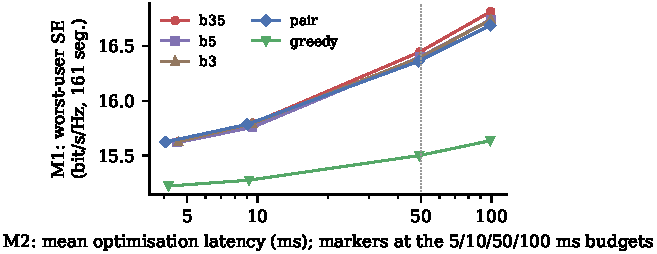
\includegraphics[width=0.62\textwidth]{figures/freespace_budget.pdf}
\caption{Controlled check: M1 against M2 for the four budgets (ME-GA, far below, omitted; see Table~\ref{tab:freespace}).}\label{fig:freespace}
\end{figure}

All five frozen contrasts are supported (Table~\ref{tab:freespace}). At 50\,ms, \bts{} exceeds exact pair search by \res{fsDBtsPairFifty}\,bit/s/Hz, wins \res{fsWinsBtsPairFifty} of \res{fsN} trajectories (\res{fsDEiBtsPairFifty} on the 81-segment mesh), and beats b3 by \res{fsDBtsBthreeFifty} and b5 by \res{fsDBtsBfiveFifty}, so each component adds to the other. Pair moves are the largest single factor: \textsc{pair} exceeds single-flip search by \res{fsDPairGreedyFifty}\,bit/s/Hz and wins all \res{fsWinsPairGreedyFifty} trajectories, while scoring \res{fsEvalsPairFifty} candidates in 50\,ms against \res{fsEvalsGreedyFifty}. The advantage of \bts{} needs time (Fig.~\ref{fig:freespace}): at 5 and 10\,ms its contrast with \textsc{pair} is \res{fsDBtsPairFive} and \res{fsDBtsPairTen}, neither supported, while at 100\,ms it grows to \res{fsDBtsPairHundred} [\res{fsLoBtsPairHundred}, \res{fsHiBtsPairHundred}]. All anytime methods use their whole budget (M2 close to M3), so quality at equal latency is the relevant comparison. ME-GA reaches \res{fsRateMegaFifty}\,bit/s/Hz at 50\,ms: it scores \res{fsEvalsMegaFifty} states (about \res{fsMegaUsPerEval}\,$\mu$s each, \res{fsMegaGenFifty} generations of \res{megaPop}), whereas \textsc{pair} scores \res{fsPairPerMegaFifty} times as many through low-rank updates. With the published population size, ME-GA completes only a few generations within tens of milliseconds.

%======================================================================
\section{Threats to Validity}\label{sec:threats}
%======================================================================
\textbf{Strength of the evolutionary baselines.} ME-GA is reimplemented from a description that leaves selection, crossover, mutation and two of its adaptive rules open; our choices are documented and fixed before any run, but a different reading could perform differently, and the published population size is not adapted to a millisecond deadline. We therefore present H2 as a comparison with the published specification, and add NSGA-II as a standard evolutionary reference on the city scope. Neither baseline exploits the low-rank structure in our implementations. A variant that rescored mutation-only offspring by low-rank updates could narrow the gap; we did not test one.

\textbf{Selection on development data.} \bts{} was chosen from an ablation ladder on development trajectories of the same free-space generator. The held-out test removes the selection bias within that distribution but not across geometries; the city scope addresses this only for one map and four sites.

\textbf{Physical model.} The surface is a free-space thin-wire model without substrate, ground plane or switch parasitics; the 161-segment mesh is a consistency check rather than a convergence proof, and the 256-element city model uses one mesh. The precoder is fixed at the all-OFF channel and full channel knowledge is assumed.

\textbf{Building-only scenes.} \res{txtBuildingOnly}

\textbf{Timing.} Deadlines are measured on one core of a lab workstation; absolute times will differ on a surface controller, but every method is timed on the same core under the same rules, so the comparison is fair at matched compute.

%======================================================================
\section{Conclusion}
%======================================================================
We proposed \bts{}, a deadline-bounded exact pair search for coupled 1-bit RIS control that scores every single and pair flip through rank-one and rank-two updates, and diversifies with predeclared restart densities and elite recombination. Under a frozen, deadline-fair protocol on a coupled method-of-moments surface, it beats exact pair search, each of its own components, and a specification-based ME-GA at a 50\,ms deadline, with the largest single improvement coming from the exact pair neighbourhood itself, and its advantage grows with the deadline. The pre-registered RIS-relevant scope of GeoRIS-Bench extends the comparison to ray-traced urban channels, larger arrays and NSGA-II.

\subsubsection*{Disclosure of Interests.} The authors have no competing interests to declare that are relevant to the content of this article.

\bibliographystyle{splncs04}
\bibliography{references}
\end{document}
